\documentclass{standalone}
\usepackage{tikz}
\usetikzlibrary{arrows.meta,positioning,fit,backgrounds,shapes.geometric,calc,shadows}

\begin{document}
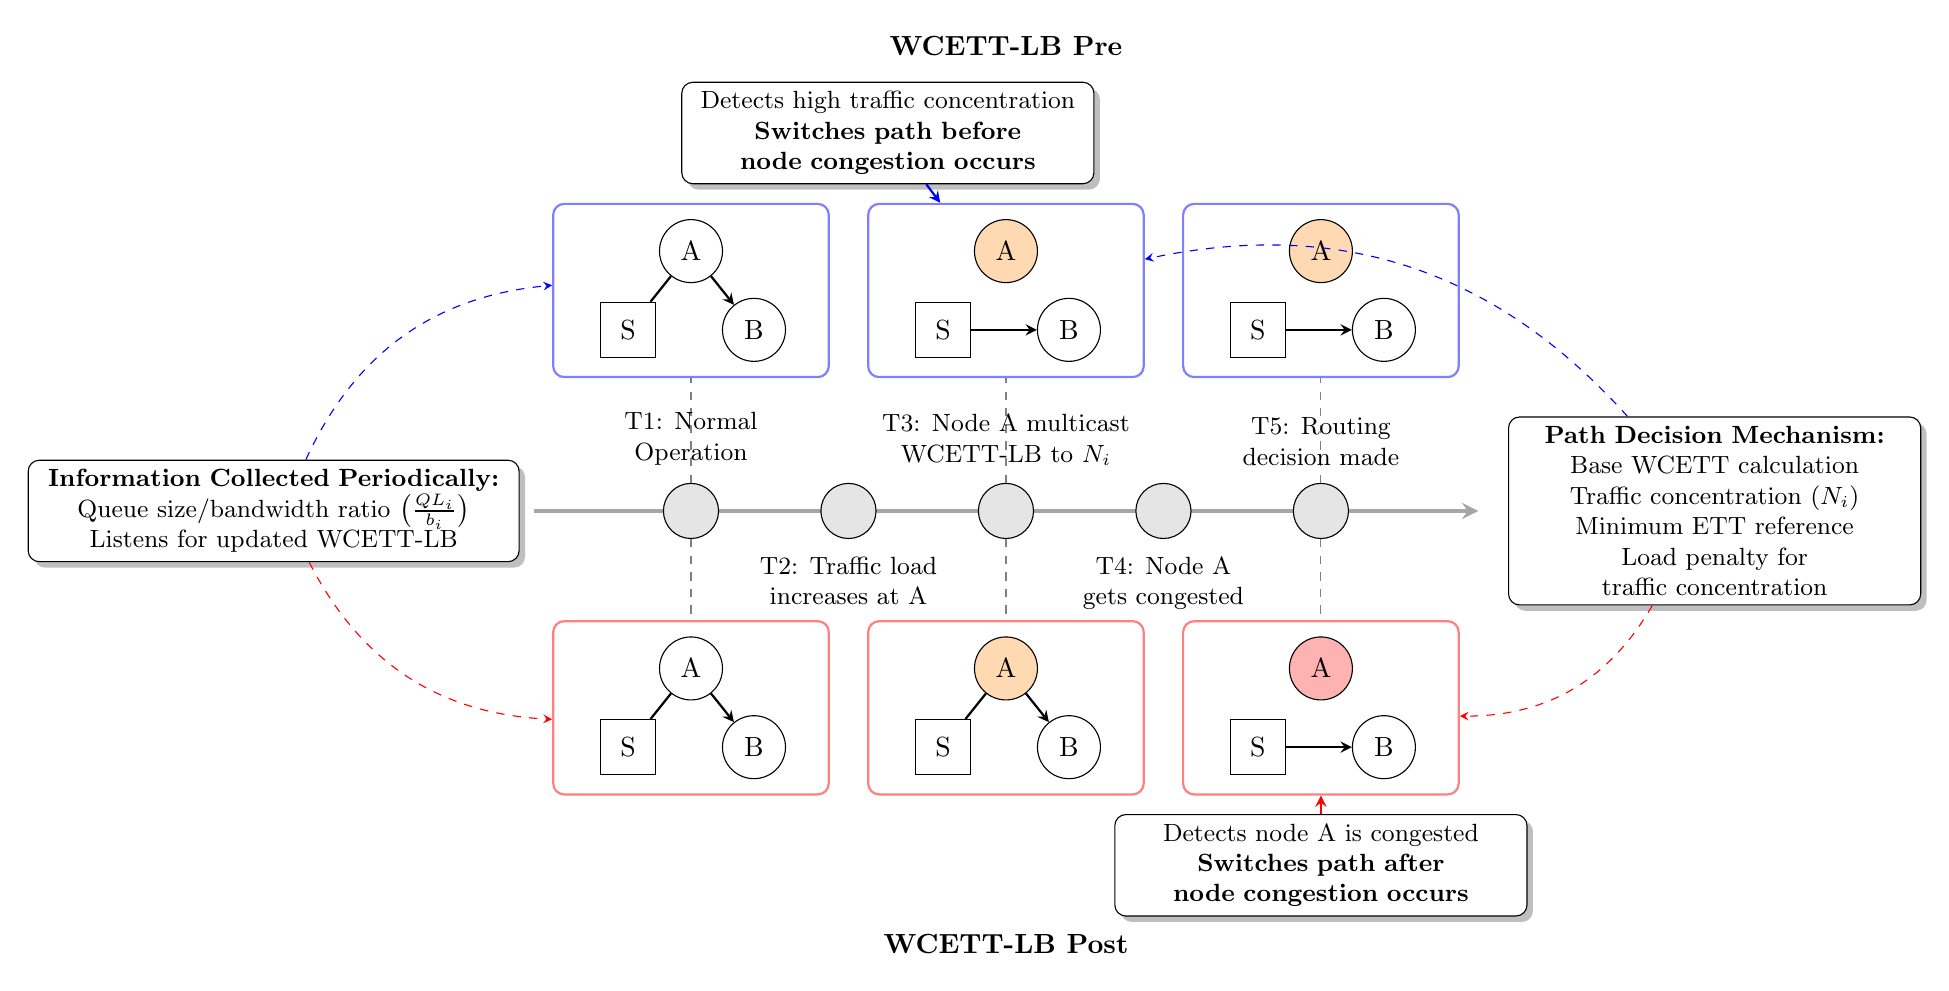
\begin{tikzpicture}[
    node distance=2cm,
    router/.style={circle, draw, minimum size=0.8cm},
    congestedrouter/.style={circle, draw, fill=red!30, minimum size=0.8cm},
    warningrouter/.style={circle, draw, fill=orange!30, minimum size=0.8cm},
    endpoint/.style={rectangle, draw, minimum size=0.7cm},
    arrow/.style={->,>=stealth, thick},
    timeline/.style={ultra thick, ->, >=stealth, draw=gray!70},
    milestone/.style={circle, draw, fill=gray!20, minimum size=0.7cm, font=\small},
    milestone_minor/.style={circle, draw, fill=gray!20, minimum size=0.7cm, font=\small},
    patharrow/.style={dashed,->,>=stealth,thick},
    infobox/.style={rectangle, draw, rounded corners, fill=white, drop shadow, align=center, text width=5cm, font=\small},
    infobox_left/.style={rectangle, draw, rounded corners, fill=white, drop shadow, align=center, text width=6cm, font=\small},
    networkbox/.style={rectangle, draw, rounded corners, minimum width=3.5cm, minimum height=2.2cm},
    label/.style={font=\small, align=center},
    title/.style={font=\bfseries, align=center}
]

% Timeline
\draw[timeline] (-1,0) -- (11,0);
\node[milestone] (t1) at (1,0) {};
\node[milestone_minor] (t2) at (3,0) {};
\node[milestone] (t3) at (5,0) {};
\node[milestone_minor] (t4) at (7,0) {};
\node[milestone] (t5) at (9,0) {};

% Pre-LB (Proactive)
\node[title] at (5,5.9) {WCETT-LB Pre};
\node[networkbox, draw=blue!50, thick] (pre1) at (1,2.8) {};
\node[networkbox, draw=blue!50, thick] (pre2) at (5,2.8) {};
\node[networkbox, draw=blue!50, thick] (pre3) at (9,2.8) {};

% Pre-LB states
\node[endpoint] (pre_s1) at ($(pre1) + (-0.8,-0.5)$) {S};
\node[router] (pre_a1) at ($(pre1) + (0,0.5)$) {A};
\node[router] (pre_b1) at ($(pre1) + (0.8,-0.5)$) {B};
\draw[arrow] (pre_s1) -- (pre_a1) -- (pre_b1);

\node[endpoint] (pre_s2) at ($(pre2) + (-0.8,-0.5)$) {S};
\node[warningrouter] (pre_a2) at ($(pre2) + (0,0.5)$) {A};
\node[router] (pre_b2) at ($(pre2) + (0.8,-0.5)$) {B};
\draw[arrow] (pre_s2) -- (pre_b2);

\node[endpoint] (pre_s3) at ($(pre3) + (-0.8,-0.5)$) {S};
\node[warningrouter] (pre_a3) at ($(pre3) + (0,0.5)$) {A};
\node[router] (pre_b3) at ($(pre3) + (0.8,-0.5)$) {B};
\draw[arrow] (pre_s3) --  (pre_b3);

\node[infobox] (pre_decision) at (3.5,4.8) {
    Detects high traffic concentration\\
    \textbf{Switches path before node congestion occurs}
};
\draw[arrow, blue] (pre_decision) to (pre2);

\node[infobox_left] (pre_info) at (-4.3,0) {
    \textbf{Information Collected Periodically:}\\
    Queue size/bandwidth ratio $\left(\frac{QL_i}{b_i}\right)$\\
    Listens for updated WCETT-LB
};
\draw[patharrow, blue, thin] (pre_info) to[bend left] (pre1);

\node[infobox] (pre_calc) at (14,0) {
    \textbf{Path Decision Mechanism:}\\
    Base WCETT calculation\\
    Traffic concentration $(N_i)$\\
    Minimum ETT reference\\
    Load penalty for\\traffic concentration
};
\draw[patharrow, blue, thin] (pre_calc) to[bend right] (pre2);

% Post-LB (Reactive)
\node[title] at (5,-5.5) {WCETT-LB Post};
\node[networkbox, draw=red!50, thick] (post1) at (1,-2.5) {};
\node[networkbox, draw=red!50, thick] (post2) at (5,-2.5) {};
\node[networkbox, draw=red!50, thick] (post3) at (9,-2.5) {};

\node[endpoint] (post_s1) at ($(post1) + (-0.8,-0.5)$) {S};
\node[router] (post_a1) at ($(post1) + (0,0.5)$) {A};
\node[router] (post_b1) at ($(post1) + (0.8,-0.5)$) {B};
\draw[arrow] (post_s1) -- (post_a1) -- (post_b1);

\node[endpoint] (post_s2) at ($(post2) + (-0.8,-0.5)$) {S};
\node[warningrouter] (post_a2) at ($(post2) + (0,0.5)$) {A};
\node[router] (post_b2) at ($(post2) + (0.8,-0.5)$) {B};
\draw[arrow] (post_s2) -- (post_a2) -- (post_b2);

\node[endpoint] (post_s3) at ($(post3) + (-0.8,-0.5)$) {S};
\node[congestedrouter] (post_a3) at ($(post3) + (0,0.5)$) {A};
\node[router] (post_b3) at ($(post3) + (0.8,-0.5)$) {B};
\draw[arrow] (post_s3) -- (post_b3);

\node[infobox] (post_decision) at (9,-4.5) {
    Detects node A is congested\\
    \textbf{Switches path after node congestion occurs}
};
\draw[arrow, red] (post_decision) to (post3);

\draw[patharrow, red, thin] (pre_info) to[bend right] (post1);
\draw[patharrow, red, thin] (pre_calc) to[bend left] (post3);

\draw[dashed, gray] (t1) -- (pre1);
\draw[dashed, gray] (t1) -- (post1);
\draw[dashed, gray] (t3) -- (pre2);
\draw[dashed, gray] (t3) -- (post2);
\draw[dashed, gray] (t5) -- (pre3);
\draw[dashed, gray] (t5) -- (post3);

\node[label, above=0.1cm of t1] {T1: Normal\\Operation};
\node[label, below=0.1cm of t2] {T2: Traffic load\\increases at A};
\node[label, above=0.1cm of t3] {T3: Node A multicast\\WCETT-LB to $N_i$};
\node[label, below=0.1cm of t4] {T4: Node A\\gets congested};
\node[label, above=0.1cm of t5] {T5: Routing\\decision made};

\end{tikzpicture}
\end{document}